\section*{Dati e risultati}

%\begin{SCfigure}[0.55][t]
%    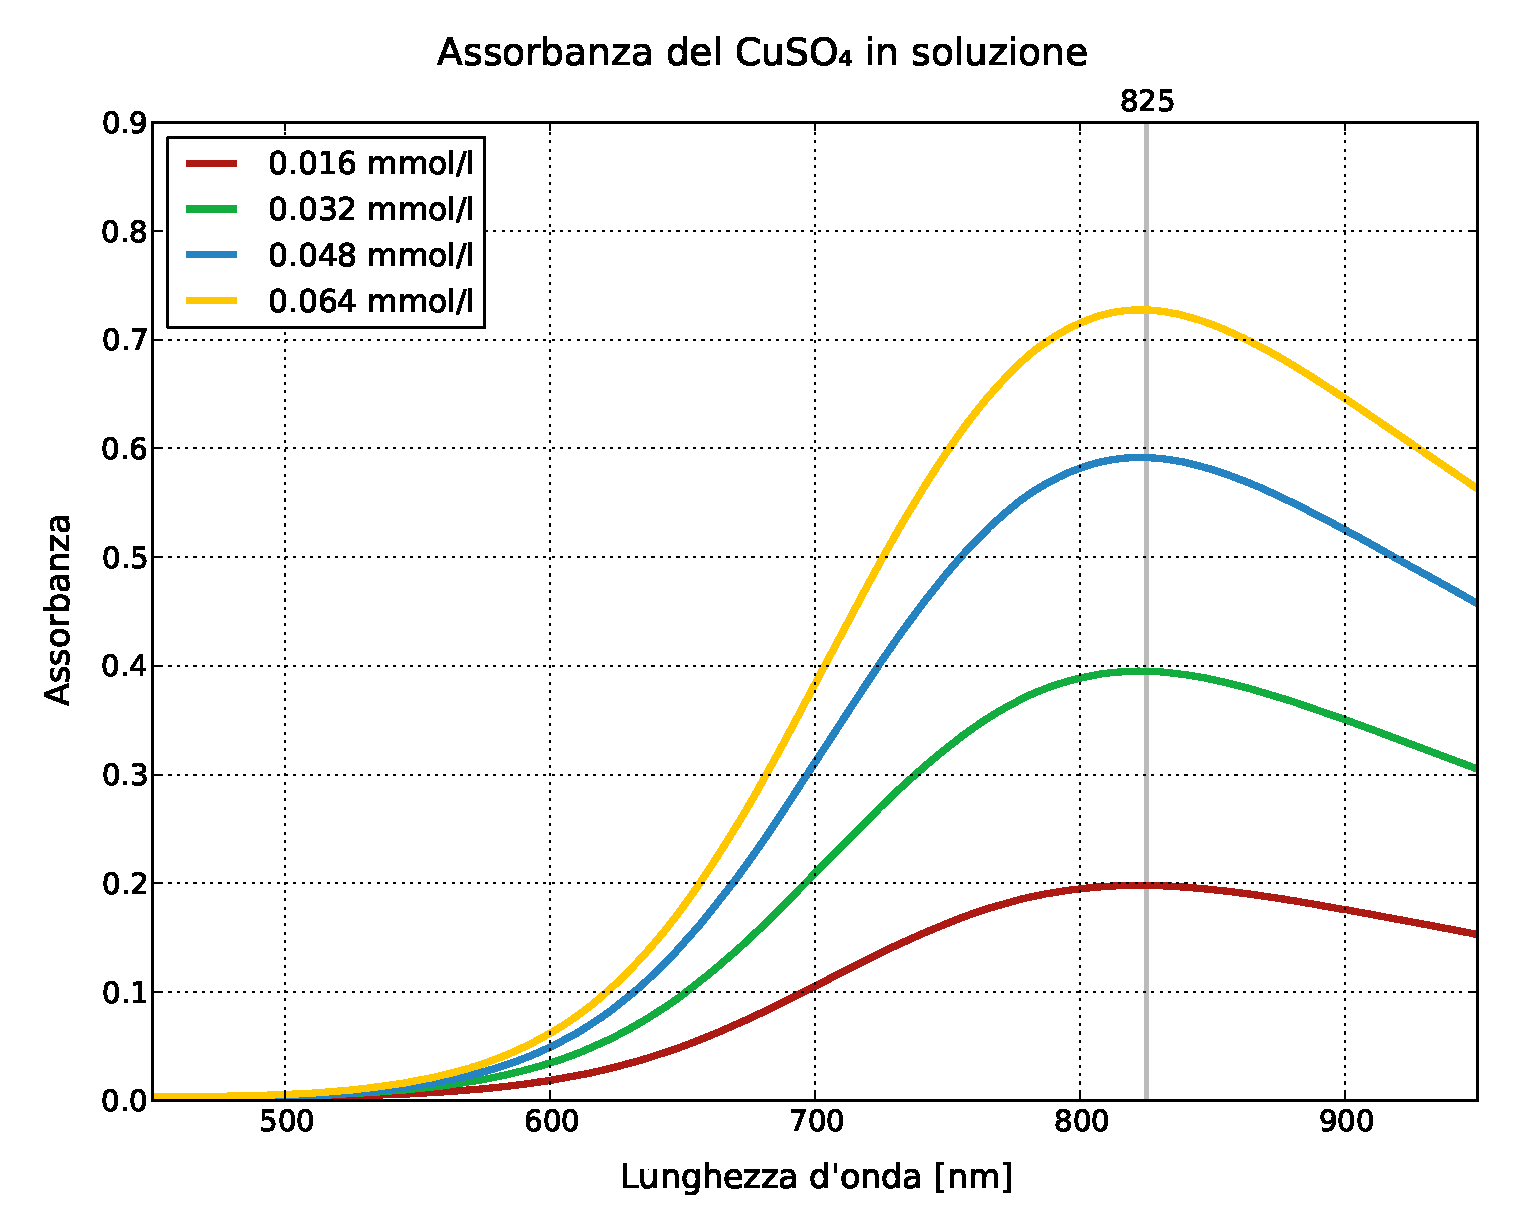
\includegraphics[scale=0.52]{concentrazioni.pdf}
%    \caption{Nel grafico sono rappresentate le curve di assorbimento in funzione della lunghezza d'onda delle quattro soluzioni note.
%        \`E stata inoltre evidenziata tramite una linea verticale la lunghezza d'onda di massima assorbanza $\lambda\ped{max} = \SI{825}{\nano\meter}$.
%        Queste curve sono interessanti poichè spiegano il colore azzurro intenso di una soluzione di \ce{CuSO4}. Il massimo di assorbimento
%        nel visibile è ad alte lunghezze d'onda, ovvero nel rosso e nell'infrarosso; la luce di colore blu invece, passa indisturbata, per cui la soluzione appare di
%        colore blu. La barra colorata in basso indica approssimativamente i colori corrispondenti alle lunghezze d'onda del grafico soprastante.}
%    \label{fig:conc}
%\end{SCfigure}

%\begin{SCfigure}[0.55][t]
%    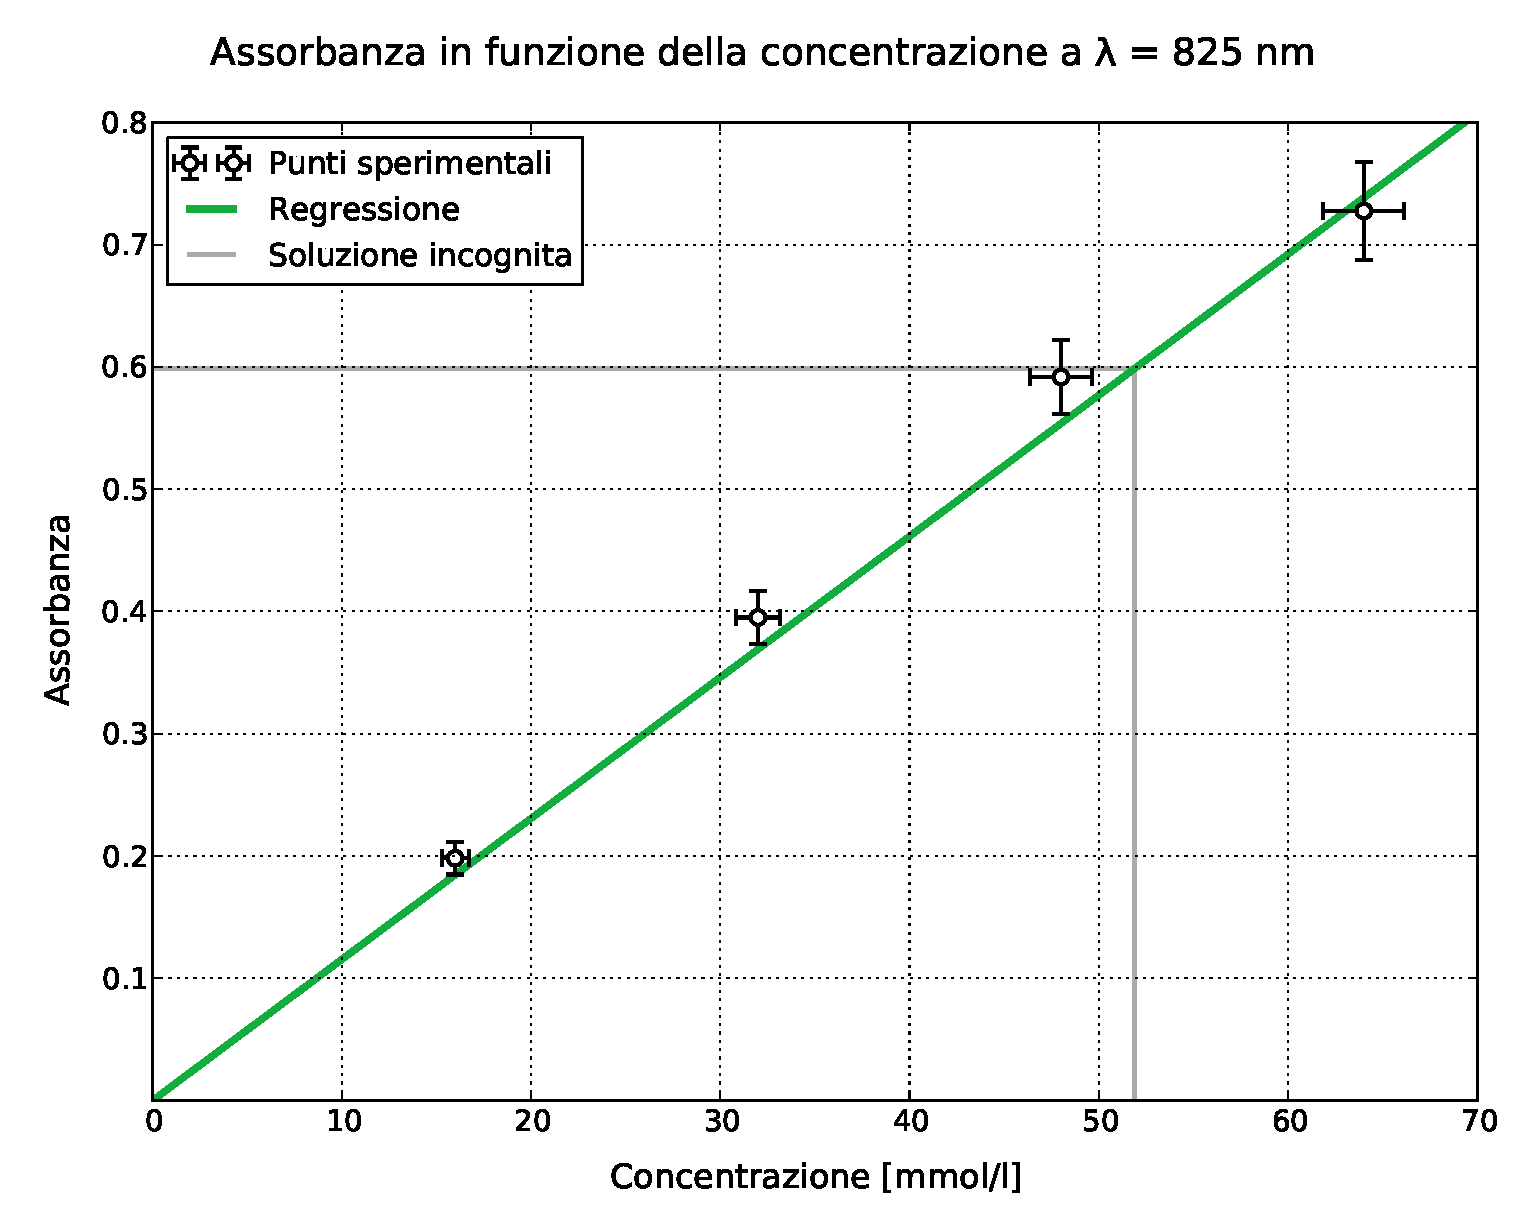
\includegraphics[scale=0.55]{retta.pdf}
%    \caption{Il grafico in figura mostra l'assorbanza a $\lambda\ped{max} = \SI{825}{nm}$ in funzione della concentrazione
%        per le quattro soluzioni preparate. Sono riportati sia gli errori sulla concentrazione, che le incertezze sull'assorbanza
%        stimate dalla correzione delle incertezze. La retta di fit in verde 
%        indica l'andamento previsto dalla legge di Lambert-Beer e ci permette di calcolare $\alpha$. In grigio è riportato
%        il valore di assorbanza della soluzione incognita, dall'intersezione con la retta di fit possiamo dire che la concentrazione
%        di tale soluzione è di circa 0.05 M.}
%    \label{fig:a_vs_c}
%\end{SCfigure}
